% Created 2017-09-11 Mon 14:46
\documentclass[9pt,lineo]{elife}

\usepackage{amsmath}
\usepackage{amssymb}
\usepackage[version=4]{mhchem}
\usepackage{siunitx}


              \usepackage[utf8]{inputenc}
\sisetup{detect-all}
\setcounter{secnumdepth}{0}
\date{\today}
\title{}
\hypersetup{
 pdfauthor={},
 pdftitle={},
 pdfkeywords={},
 pdfsubject={},
 pdfcreator={Emacs 25.1.2 (Org mode 8.3.5)}, 
 pdflang={English}}
\begin{document}

\begin{figure}
\begin{fullwidth}
\centering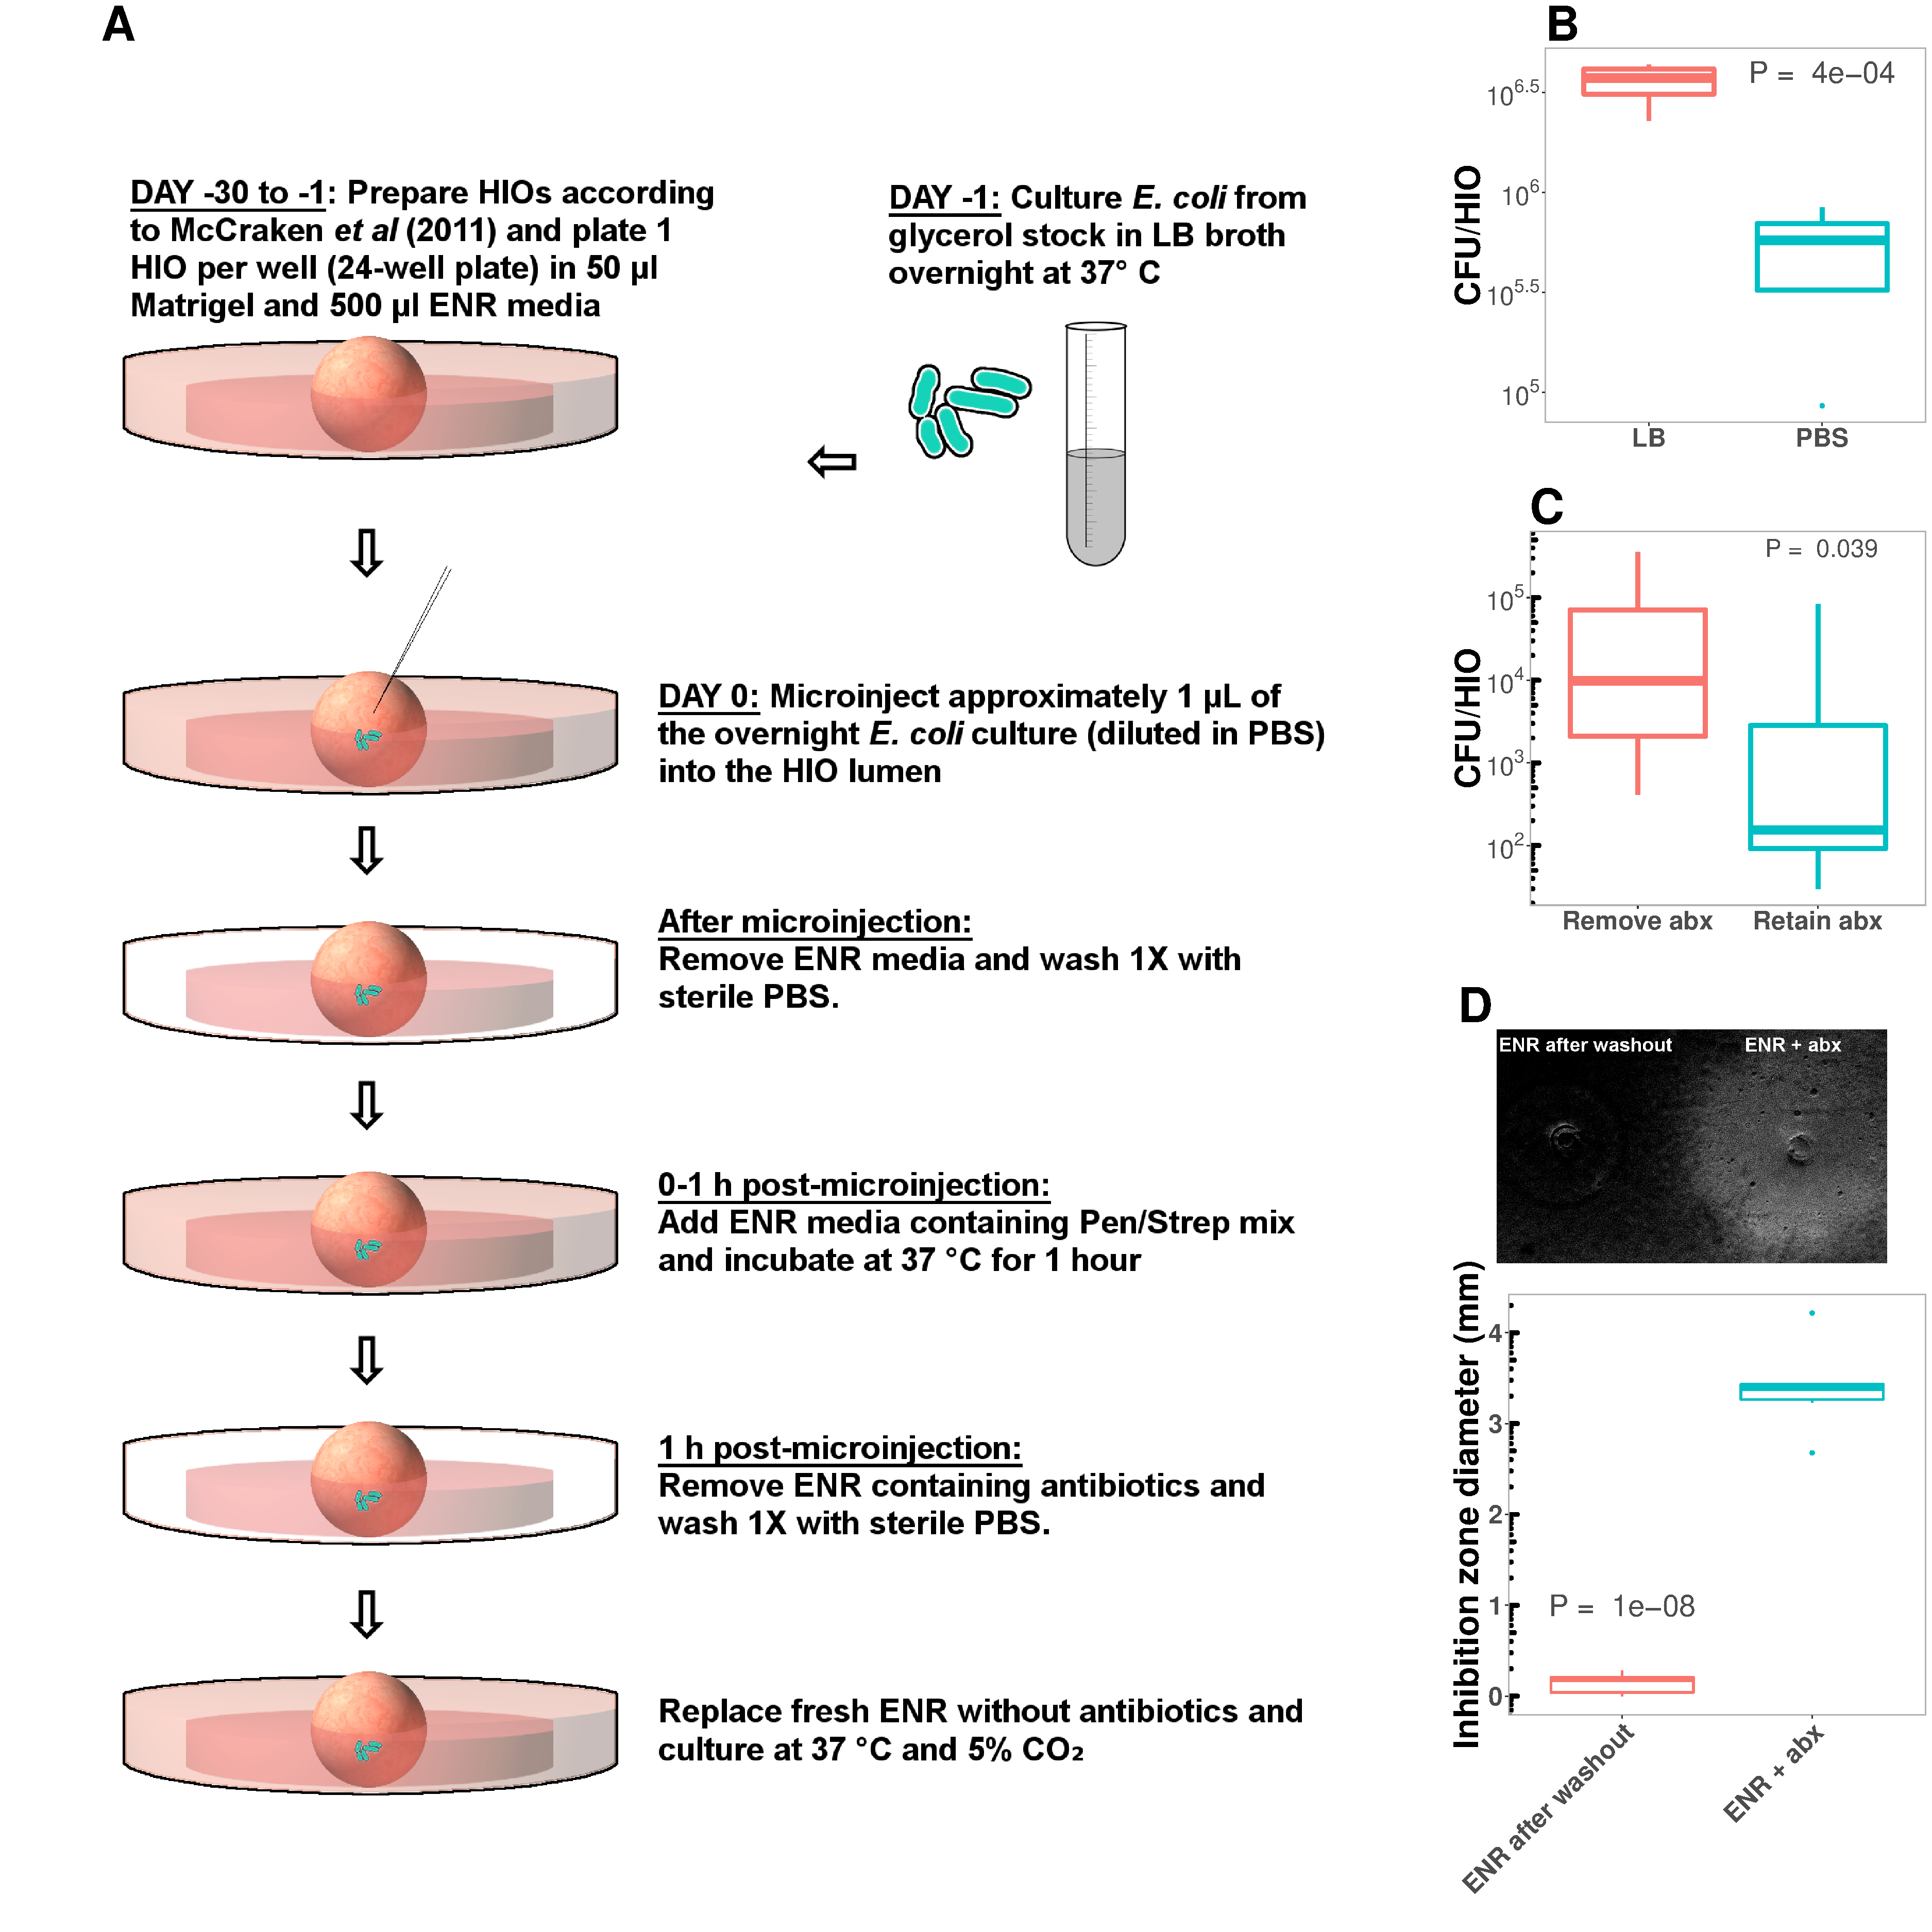
\includegraphics[width=0.85\linewidth]{./figures/figure1/sfigure1-3_multipanel.pdf}
\caption*{\textbf{Figure 1 - Supplement 3. } \textbf{A} Schematic representation of the microinjection of HIOs with live \textit{E. coli}. See Materials and Methods for additional details. \textbf{B} A comparison of CFU/HIO at 24 h post-microinjection of HIOs microinjected with \num{10e3} CFU live \textit{E. coli} diluted in sterile PBS or fresh LB broth. \textit{n} = 5 HIOs per condition. All experiments presented in the main paper represent \textit{E. coli} diluted in PBS. \textit{C} To test for the effect of antibiotic carryover of \textit{E. coli} growth in the HIO lumen, we compared CFU/HIO in HIOs cultured in antibiotic free media ("Remove abx") or media containing penicillin and streptomycin at 24 h post-microinjection with \num{10e3} CFU live \textit{E. coli}. All experiments presented in the main paper represent HIOs cultured in antibiotic-free media due to the apparent effect of antibiotics in suppressing \textit{E. coli} growth within the HIO lumen. \textit{n} = 5 HIOs per condition. \textit{D} In several experiments, bacterial translocation was measured by samplign the external HIO culture media (Figures 1 and 8). To evaluate the potential influence of antibiotic carryover in our estimates of bacterial translocation, we measured growth inhibition in \textit{E. coli} cultures plated as a lawn of LB agar and treated with 1 $\mu$l samples of HIO media collected during the 1 h antibiotic wash step or after HIO culture washout with PBS and replacement with fresh antibiotic free media (see panel A). \textit{n} = 6 replicates per culture condition. All \textit{P}-values represent the results of unpaired one-tailed Student's \textit{t}-test comparisons.}
\label{fig:fullwidth}
\end{fullwidth}
\end{figure}
\end{document}